\documentclass[twoside]{book}

% Packages required by doxygen
\usepackage{fixltx2e}
\usepackage{calc}
\usepackage{doxygen}
\usepackage[export]{adjustbox} % also loads graphicx
\usepackage{graphicx}
\usepackage[utf8]{inputenc}
\usepackage{makeidx}
\usepackage{multicol}
\usepackage{multirow}
\PassOptionsToPackage{warn}{textcomp}
\usepackage{textcomp}
\usepackage[nointegrals]{wasysym}
\usepackage[table]{xcolor}

% Font selection
\usepackage[T1]{fontenc}
\usepackage[scaled=.90]{helvet}
\usepackage{courier}
\usepackage{amssymb}
\usepackage{sectsty}
\renewcommand{\familydefault}{\sfdefault}
\allsectionsfont{%
  \fontseries{bc}\selectfont%
  \color{darkgray}%
}
\renewcommand{\DoxyLabelFont}{%
  \fontseries{bc}\selectfont%
  \color{darkgray}%
}
\newcommand{\+}{\discretionary{\mbox{\scriptsize$\hookleftarrow$}}{}{}}

% Page & text layout
\usepackage{geometry}
\geometry{%
  a4paper,%
  top=2.5cm,%
  bottom=2.5cm,%
  left=2.5cm,%
  right=2.5cm%
}
\tolerance=750
\hfuzz=15pt
\hbadness=750
\setlength{\emergencystretch}{15pt}
\setlength{\parindent}{0cm}
\setlength{\parskip}{3ex plus 2ex minus 2ex}
\makeatletter
\renewcommand{\paragraph}{%
  \@startsection{paragraph}{4}{0ex}{-1.0ex}{1.0ex}{%
    \normalfont\normalsize\bfseries\SS@parafont%
  }%
}
\renewcommand{\subparagraph}{%
  \@startsection{subparagraph}{5}{0ex}{-1.0ex}{1.0ex}{%
    \normalfont\normalsize\bfseries\SS@subparafont%
  }%
}
\makeatother

% Headers & footers
\usepackage{fancyhdr}
\pagestyle{fancyplain}
\fancyhead[LE]{\fancyplain{}{\bfseries\thepage}}
\fancyhead[CE]{\fancyplain{}{}}
\fancyhead[RE]{\fancyplain{}{\bfseries\leftmark}}
\fancyhead[LO]{\fancyplain{}{\bfseries\rightmark}}
\fancyhead[CO]{\fancyplain{}{}}
\fancyhead[RO]{\fancyplain{}{\bfseries\thepage}}
\fancyfoot[LE]{\fancyplain{}{}}
\fancyfoot[CE]{\fancyplain{}{}}
\fancyfoot[RE]{\fancyplain{}{\bfseries\scriptsize Generated by Doxygen }}
\fancyfoot[LO]{\fancyplain{}{\bfseries\scriptsize Generated by Doxygen }}
\fancyfoot[CO]{\fancyplain{}{}}
\fancyfoot[RO]{\fancyplain{}{}}
\renewcommand{\footrulewidth}{0.4pt}
\renewcommand{\chaptermark}[1]{%
  \markboth{#1}{}%
}
\renewcommand{\sectionmark}[1]{%
  \markright{\thesection\ #1}%
}

% Indices & bibliography
\usepackage{natbib}
\usepackage[titles]{tocloft}
\setcounter{tocdepth}{3}
\setcounter{secnumdepth}{5}
\makeindex

% Hyperlinks (required, but should be loaded last)
\usepackage{ifpdf}
\ifpdf
  \usepackage[pdftex,pagebackref=true]{hyperref}
\else
  \usepackage[ps2pdf,pagebackref=true]{hyperref}
\fi
\hypersetup{%
  colorlinks=true,%
  linkcolor=blue,%
  citecolor=blue,%
  unicode%
}

% Custom commands
\newcommand{\clearemptydoublepage}{%
  \newpage{\pagestyle{empty}\cleardoublepage}%
}

\usepackage{caption}
\captionsetup{labelsep=space,justification=centering,font={bf},singlelinecheck=off,skip=4pt,position=top}

%===== C O N T E N T S =====

\begin{document}

% Titlepage & ToC
\hypersetup{pageanchor=false,
             bookmarksnumbered=true,
             pdfencoding=unicode
            }
\pagenumbering{roman}
\begin{titlepage}
\vspace*{7cm}
\begin{center}%
{\Large Stbx\+Engine }\\
\vspace*{1cm}
{\large Generated by Doxygen 1.8.11}\\
\end{center}
\end{titlepage}
\clearemptydoublepage
\tableofcontents
\clearemptydoublepage
\pagenumbering{arabic}
\hypersetup{pageanchor=true}

%--- Begin generated contents ---
\chapter{Hierarchical Index}
\section{Class Hierarchy}
This inheritance list is sorted roughly, but not completely, alphabetically\+:\begin{DoxyCompactList}
\item \contentsline{section}{Console}{\pageref{classConsole}}{}
\item \contentsline{section}{Control}{\pageref{classControl}}{}
\item \contentsline{section}{Engine}{\pageref{classEngine}}{}
\item \contentsline{section}{Keybinds}{\pageref{classKeybinds}}{}
\item \contentsline{section}{Menu}{\pageref{classMenu}}{}
\item \contentsline{section}{Menu\+Item}{\pageref{classMenuItem}}{}
\begin{DoxyCompactList}
\item \contentsline{section}{Menu\+Edit}{\pageref{classMenuEdit}}{}
\item \contentsline{section}{Menu\+Link}{\pageref{classMenuLink}}{}
\item \contentsline{section}{Menu\+Setting}{\pageref{classMenuSetting}}{}
\begin{DoxyCompactList}
\item \contentsline{section}{Menu\+Dynamic\+Setting}{\pageref{classMenuDynamicSetting}}{}
\end{DoxyCompactList}
\item \contentsline{section}{Menu\+Slider}{\pageref{classMenuSlider}}{}
\end{DoxyCompactList}
\end{DoxyCompactList}

\chapter{Class Index}
\section{Class List}
Here are the classes, structs, unions and interfaces with brief descriptions\+:\begin{DoxyCompactList}
\item\contentsline{section}{\hyperlink{classConsole}{Console} \\*Integrated toggleable developer console }{\pageref{classConsole}}{}
\item\contentsline{section}{\hyperlink{classControl}{Control} \\*Key, or Mouse event }{\pageref{classControl}}{}
\item\contentsline{section}{\hyperlink{classEngine}{Engine} \\*Main class for graphic conception }{\pageref{classEngine}}{}
\item\contentsline{section}{\hyperlink{classKeybinds}{Keybinds} \\*Dictionnary of current bound keys at runtime }{\pageref{classKeybinds}}{}
\item\contentsline{section}{\hyperlink{classMenu}{Menu} \\*Simple class for generating menus }{\pageref{classMenu}}{}
\item\contentsline{section}{\hyperlink{classMenuDynamicSetting}{Menu\+Dynamic\+Setting} \\*Dynamic Setting item, showing a list of values known only at runtime }{\pageref{classMenuDynamicSetting}}{}
\item\contentsline{section}{\hyperlink{classMenuEdit}{Menu\+Edit} \\*Input box, either used for key binding, or text input from user }{\pageref{classMenuEdit}}{}
\item\contentsline{section}{\hyperlink{classMenuItem}{Menu\+Item} \\*Abstract \hyperlink{classMenu}{Menu} item }{\pageref{classMenuItem}}{}
\item\contentsline{section}{\hyperlink{classMenuLink}{Menu\+Link} \\*\hyperlink{classMenu}{Menu} link to another menu or action }{\pageref{classMenuLink}}{}
\item\contentsline{section}{\hyperlink{classMenuSetting}{Menu\+Setting} \\*Static Setting item, showing a list of values defined in X\+ML }{\pageref{classMenuSetting}}{}
\item\contentsline{section}{\hyperlink{classMenuSlider}{Menu\+Slider} \\*Slider Setting item, accept any value within defined range }{\pageref{classMenuSlider}}{}
\end{DoxyCompactList}

\chapter{File Index}
\section{File List}
Here is a list of all documented files with brief descriptions\+:\begin{DoxyCompactList}
\item\contentsline{section}{include/\hyperlink{Commands_8hh}{Commands.\+hh} \\*Contains definition of basic console commands }{\pageref{Commands_8hh}}{}
\item\contentsline{section}{include/\hyperlink{Console_8hh}{Console.\+hh} }{\pageref{Console_8hh}}{}
\item\contentsline{section}{include/\hyperlink{Control_8hh}{Control.\+hh} }{\pageref{Control_8hh}}{}
\item\contentsline{section}{include/\hyperlink{Engine_8hpp}{Engine.\+hpp} }{\pageref{Engine_8hpp}}{}
\item\contentsline{section}{include/\hyperlink{Keybinds_8hh}{Keybinds.\+hh} }{\pageref{Keybinds_8hh}}{}
\item\contentsline{section}{include/\hyperlink{Menu_8hh}{Menu.\+hh} }{\pageref{Menu_8hh}}{}
\item\contentsline{section}{include/\hyperlink{MenuItem_8hh}{Menu\+Item.\+hh} \\*\hyperlink{classMenu}{Menu} items (links, settings, sliders, text inputs, ...) }{\pageref{MenuItem_8hh}}{}
\end{DoxyCompactList}

\chapter{Class Documentation}
\hypertarget{classConsole}{}\section{Console Class Reference}
\label{classConsole}\index{Console@{Console}}


Integrated toggleable developer console.  




{\ttfamily \#include $<$Console.\+hh$>$}

\subsection*{Public Member Functions}
\begin{DoxyCompactItemize}
\item 
{\bfseries Console} (\hyperlink{classEngine}{Engine} \&e)\hypertarget{classConsole_ae948623138ea20074160fc8004cda111}{}\label{classConsole_ae948623138ea20074160fc8004cda111}

\item 
void {\bfseries init\+Graphics} (const sf\+::\+Vector2i \&winsize)\hypertarget{classConsole_af62ee9b064c2a7b5e2d3458cdfd98bbe}{}\label{classConsole_af62ee9b064c2a7b5e2d3458cdfd98bbe}

\item 
void {\bfseries toggle} ()\hypertarget{classConsole_ad0fb3ae7fe0f21999c71a138421bd0be}{}\label{classConsole_ad0fb3ae7fe0f21999c71a138421bd0be}

\item 
void {\bfseries clear} ()\hypertarget{classConsole_a8b4ffaeabbea48e1f3aa1e535ee88ab8}{}\label{classConsole_a8b4ffaeabbea48e1f3aa1e535ee88ab8}

\item 
bool {\bfseries is\+Active} () const \hypertarget{classConsole_a3b9de7e1192338c516570c1753dcba6a}{}\label{classConsole_a3b9de7e1192338c516570c1753dcba6a}

\item 
void {\bfseries set\+Line\+Count} (const unsigned int \&count)\hypertarget{classConsole_a7b2e6d42de564cea813229c6bd8f07ae}{}\label{classConsole_a7b2e6d42de564cea813229c6bd8f07ae}

\item 
void {\bfseries set\+Color} (sf\+::\+Color bg, sf\+::\+Color input)\hypertarget{classConsole_a3630b0f354654ef69551c91cbfe07b8f}{}\label{classConsole_a3630b0f354654ef69551c91cbfe07b8f}

\item 
void {\bfseries set\+Cursor} (char \&c)\hypertarget{classConsole_a7a7db54bbcf057da981adfc06c352e64}{}\label{classConsole_a7a7db54bbcf057da981adfc06c352e64}

\item 
void {\bfseries set\+Log\+Enabled} (bool state)\hypertarget{classConsole_ab73eef5e22ab9ef218dc63433fc418fa}{}\label{classConsole_ab73eef5e22ab9ef218dc63433fc418fa}

\item 
void {\bfseries write\+To\+Log} (std\+::string \&msg)\hypertarget{classConsole_a555537aaa8a953d0459efb2392eb74ac}{}\label{classConsole_a555537aaa8a953d0459efb2392eb74ac}

\item 
void {\bfseries set\+Log\+File} (const std\+::string \&file)\hypertarget{classConsole_ae135a01de6429f545532b933baf3c677}{}\label{classConsole_ae135a01de6429f545532b933baf3c677}

\item 
void {\bfseries set\+Log\+Timestamp} (int)\hypertarget{classConsole_a2063152a09b8fc481402fa2b91acf435}{}\label{classConsole_a2063152a09b8fc481402fa2b91acf435}

\item 
void {\bfseries output} (std\+::string msg)\hypertarget{classConsole_ae77795030b9a6f37f9745973d82176ef}{}\label{classConsole_ae77795030b9a6f37f9745973d82176ef}

\item 
void {\bfseries output} (std\+::string color, std\+::string msg)\hypertarget{classConsole_aacfc9448be616fd4459699db7a635551}{}\label{classConsole_aacfc9448be616fd4459699db7a635551}

\item 
void {\bfseries insert\+Last\+Output} (const std\+::string \&msg)\hypertarget{classConsole_ac8da15dab46dad5dc3c27fb8687a5fa9}{}\label{classConsole_ac8da15dab46dad5dc3c27fb8687a5fa9}

\item 
void {\bfseries input} ()\hypertarget{classConsole_a50056cdeafd8ccf150f3f7e00d077ff5}{}\label{classConsole_a50056cdeafd8ccf150f3f7e00d077ff5}

\item 
void {\bfseries update\+Input} (const sf\+::\+Event \&event)\hypertarget{classConsole_ae58f6f060dd09567347cfc6b00b923fa}{}\label{classConsole_ae58f6f060dd09567347cfc6b00b923fa}

\item 
void {\bfseries update\+Input\+Value} ()\hypertarget{classConsole_a78097e40392c525d82c77506ba501e7b}{}\label{classConsole_a78097e40392c525d82c77506ba501e7b}

\item 
void {\bfseries update\+Output} ()\hypertarget{classConsole_a4f513601e3fed552f8999ef8ec99ff02}{}\label{classConsole_a4f513601e3fed552f8999ef8ec99ff02}

\item 
void {\bfseries update\+Keyboard} (const sf\+::\+Event \&event)\hypertarget{classConsole_a5d3acb9de22bb5de6475431cb7dfa4e9}{}\label{classConsole_a5d3acb9de22bb5de6475431cb7dfa4e9}

\item 
void {\bfseries update} (const sf\+::\+Event \&event)\hypertarget{classConsole_aa5303865edd868a23c7cf77795bc9d4e}{}\label{classConsole_aa5303865edd868a23c7cf77795bc9d4e}

\item 
void {\bfseries draw} (sf\+::\+Render\+Window $\ast$win)\hypertarget{classConsole_a3521a7d331b2224e2034b079caeed4c2}{}\label{classConsole_a3521a7d331b2224e2034b079caeed4c2}

\end{DoxyCompactItemize}
\subsection*{Static Public Member Functions}
\begin{DoxyCompactItemize}
\item 
static sf\+::\+Color {\bfseries convert\+Color\+Code} (std\+::string code, std\+::string esc=\char`\"{}\textbackslash{}\textbackslash{}\textbackslash{}\textbackslash{}\#\char`\"{})\hypertarget{classConsole_a562839a9b9607484329523d4910b0cd6}{}\label{classConsole_a562839a9b9607484329523d4910b0cd6}

\end{DoxyCompactItemize}


\subsection{Detailed Description}
Integrated toggleable developer console. 

This console is designed to provide to developer and advanced users a way to easily configure the engine the way they want, by allowing anything that the \hyperlink{classEngine}{Engine} support to be altered by a command including keybinds, and graphical properties. 

The documentation for this class was generated from the following file\+:\begin{DoxyCompactItemize}
\item 
include/\hyperlink{Console_8hh}{Console.\+hh}\end{DoxyCompactItemize}

\hypertarget{classControl}{}\section{Control Class Reference}
\label{classControl}\index{Control@{Control}}


Key, or Mouse event.  




{\ttfamily \#include $<$Control.\+hh$>$}

\subsection*{Public Member Functions}
\begin{DoxyCompactItemize}
\item 
{\bfseries Control} (std\+::string)\hypertarget{classControl_a94fc7a98ac5b7a2121a8520a1395a3e4}{}\label{classControl_a94fc7a98ac5b7a2121a8520a1395a3e4}

\item 
{\bfseries Control} (std\+::string, const sf\+::\+Keyboard\+::\+Key key)\hypertarget{classControl_ae5830eb149d23f9b53b39323615d072d}{}\label{classControl_ae5830eb149d23f9b53b39323615d072d}

\item 
{\bfseries Control} (std\+::string, const sf\+::\+Mouse\+::\+Button btn)\hypertarget{classControl_a5d6af9adbe94c641806c6f946977ec8f}{}\label{classControl_a5d6af9adbe94c641806c6f946977ec8f}

\item 
{\bfseries Control} (std\+::string, const int whl)\hypertarget{classControl_a0161c7575f3cf302b4b4ba6161d6d318}{}\label{classControl_a0161c7575f3cf302b4b4ba6161d6d318}

\item 
{\bfseries Control} (const \hyperlink{classControl}{Control} \&c)\hypertarget{classControl_ae1520bca9129f40109cb5c0ef9835c52}{}\label{classControl_ae1520bca9129f40109cb5c0ef9835c52}

\item 
std\+::string {\bfseries get\+Bind\+Str} () const \hypertarget{classControl_a1f4f24fadb60842dffff80b714bf7ed8}{}\label{classControl_a1f4f24fadb60842dffff80b714bf7ed8}

\item 
bool {\bfseries is\+Triggered} (const sf\+::\+Event \&e)\hypertarget{classControl_ab58dcc314a5f88e2f49a78d5f4e29400}{}\label{classControl_ab58dcc314a5f88e2f49a78d5f4e29400}

\item 
bool {\bfseries is\+Released} (const sf\+::\+Event \&e)\hypertarget{classControl_a2b1d44aea6bc5adafceb7c0bc6b4820f}{}\label{classControl_a2b1d44aea6bc5adafceb7c0bc6b4820f}

\end{DoxyCompactItemize}
\subsection*{Static Public Attributes}
\begin{DoxyCompactItemize}
\item 
static std\+::map$<$ std\+::string, \hyperlink{classControl}{Control} $>$ {\bfseries keys}\hypertarget{classControl_a7688105cfe0c914511b1b4fb0e349984}{}\label{classControl_a7688105cfe0c914511b1b4fb0e349984}

\end{DoxyCompactItemize}
\subsection*{Friends}
\begin{DoxyCompactItemize}
\item 
bool {\bfseries operator==} (const \hyperlink{classControl}{Control} \&a, const \hyperlink{classControl}{Control} \&b)\hypertarget{classControl_a8f2855510a7bf0d1dfdf52351cc33087}{}\label{classControl_a8f2855510a7bf0d1dfdf52351cc33087}

\item 
bool {\bfseries operator$<$} (const \hyperlink{classControl}{Control} \&a, const \hyperlink{classControl}{Control} \&b)\hypertarget{classControl_aa607f41e48fdeaa5bcfe905f3fda5125}{}\label{classControl_aa607f41e48fdeaa5bcfe905f3fda5125}

\end{DoxyCompactItemize}


\subsection{Detailed Description}
Key, or Mouse event. 

This class is a layer above S\+F\+ML Controls, allowing usage of mouse and keyboard events generically, thanks to the implementation of generic callbacks at top level. 

The documentation for this class was generated from the following file\+:\begin{DoxyCompactItemize}
\item 
include/\hyperlink{Control_8hh}{Control.\+hh}\end{DoxyCompactItemize}

\hypertarget{classEngine}{}\section{Engine Class Reference}
\label{classEngine}\index{Engine@{Engine}}


Main class for graphic conception.  




{\ttfamily \#include $<$Engine.\+hpp$>$}



Collaboration diagram for Engine\+:\nopagebreak
\begin{figure}[H]
\begin{center}
\leavevmode
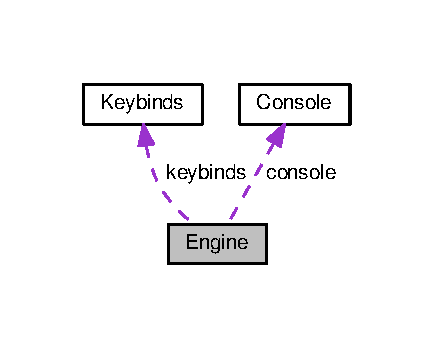
\includegraphics[width=208pt]{classEngine__coll__graph}
\end{center}
\end{figure}
\subsection*{Public Member Functions}
\begin{DoxyCompactItemize}
\item 
{\bfseries Engine} (int width=800, int height=600)\hypertarget{classEngine_a584a47606683775104df9f2482658c22}{}\label{classEngine_a584a47606683775104df9f2482658c22}

\item 
bool {\bfseries open\+Window} (int, int)\hypertarget{classEngine_ac871cb91c5e3e89a393f8f949019cd2c}{}\label{classEngine_ac871cb91c5e3e89a393f8f949019cd2c}

\item 
sf\+::\+Vector2i {\bfseries get\+Window\+Size} () const \hypertarget{classEngine_ab9d1278fde66c010cba3b844a54867af}{}\label{classEngine_ab9d1278fde66c010cba3b844a54867af}

\item 
void {\bfseries handle\+Args} (int argc, char $\ast$$\ast$argv)\hypertarget{classEngine_a3b43df5b91bc06fa908d6a55d5f40b7d}{}\label{classEngine_a3b43df5b91bc06fa908d6a55d5f40b7d}

\item 
void {\bfseries video\+Param\+Set} (const std\+::string \&, const int \&)\hypertarget{classEngine_ab3f36faf089353dc0d020354d762788e}{}\label{classEngine_ab3f36faf089353dc0d020354d762788e}

\item 
sf\+::\+Image {\bfseries capture} ()\hypertarget{classEngine_abffb4aa8da34832c14c7b041b1c864b8}{}\label{classEngine_abffb4aa8da34832c14c7b041b1c864b8}

\item 
void {\bfseries graphics\+Loop} ()\hypertarget{classEngine_a8e0654bb674af345b9f7ca3f31219ec2}{}\label{classEngine_a8e0654bb674af345b9f7ca3f31219ec2}

\item 
virtual void {\bfseries draw} ()=0\hypertarget{classEngine_a04f3ee9b4ddc0d67406536a2fe525f31}{}\label{classEngine_a04f3ee9b4ddc0d67406536a2fe525f31}

\item 
bool {\bfseries update\+Loop} ()\hypertarget{classEngine_a6a34f4802fa7e66008518bc4e89e54d9}{}\label{classEngine_a6a34f4802fa7e66008518bc4e89e54d9}

\item 
virtual bool {\bfseries update} (sf\+::\+Event \&)=0\hypertarget{classEngine_a4d52da4c5d8620de700f4f19caf7b160}{}\label{classEngine_a4d52da4c5d8620de700f4f19caf7b160}

\item 
int {\bfseries main\+Loop} ()\hypertarget{classEngine_a100911d0f2947bf8a9a9273002da25e6}{}\label{classEngine_a100911d0f2947bf8a9a9273002da25e6}

\item 
void {\bfseries quit} ()\hypertarget{classEngine_abd6e5ae9f755e283f4cc6b69ab24c582}{}\label{classEngine_abd6e5ae9f755e283f4cc6b69ab24c582}

\end{DoxyCompactItemize}
\subsection*{Static Public Member Functions}
\begin{DoxyCompactItemize}
\item 
static char {\bfseries get\+Char} (sf\+::\+Event event, Char\+Type type, bool use\+Binds=true)\hypertarget{classEngine_a8de2605cee789558ae211e4fac46b5e1}{}\label{classEngine_a8de2605cee789558ae211e4fac46b5e1}

\item 
static struct tm $\ast$ {\bfseries get\+Time} ()\hypertarget{classEngine_afb9db1b96d86458ae665b2614fd0bd9b}{}\label{classEngine_afb9db1b96d86458ae665b2614fd0bd9b}

\item 
static std\+::string {\bfseries get\+Timestamp} ()\hypertarget{classEngine_ad89df061e48c5dfb14632b67fc77fe0c}{}\label{classEngine_ad89df061e48c5dfb14632b67fc77fe0c}

\end{DoxyCompactItemize}
\subsection*{Static Public Attributes}
\begin{DoxyCompactItemize}
\item 
static \hyperlink{classKeybinds}{Keybinds} $\ast$ {\bfseries keybinds}\hypertarget{classEngine_a8a8da9ed9351a24a655f86b5bec194d3}{}\label{classEngine_a8a8da9ed9351a24a655f86b5bec194d3}

\item 
static \hyperlink{classConsole}{Console} $\ast$ {\bfseries console}\hypertarget{classEngine_a53c45cdb8fb792675360bcd126a11c55}{}\label{classEngine_a53c45cdb8fb792675360bcd126a11c55}

\end{DoxyCompactItemize}


\subsection{Detailed Description}
Main class for graphic conception. 

This the base class of the project. You must inherit from this class to start using the graphic engine. Start by implementing the update and draw routine, related to the behaviour you expect in your game. In your main function, simply instantiate your child \hyperlink{classEngine}{Engine}, then call the main\+Loop method to start the program. 

The documentation for this class was generated from the following file\+:\begin{DoxyCompactItemize}
\item 
include/\hyperlink{Engine_8hpp}{Engine.\+hpp}\end{DoxyCompactItemize}

\hypertarget{classKeybinds}{}\section{Keybinds Class Reference}
\label{classKeybinds}\index{Keybinds@{Keybinds}}


Dictionnary of current bound keys at runtime.  




{\ttfamily \#include $<$Keybinds.\+hh$>$}

\subsection*{Public Member Functions}
\begin{DoxyCompactItemize}
\item 
void {\bfseries bind\+Env} (\hyperlink{classEngine}{Engine} $\ast$)\hypertarget{classKeybinds_a5c4adba1761c402fbaeb420581d8129a}{}\label{classKeybinds_a5c4adba1761c402fbaeb420581d8129a}

\item 
bool {\bfseries is\+Bound} (const \hyperlink{classControl}{Control} \&c)\hypertarget{classKeybinds_aea000ffe6db05fc86ae7b633789995d4}{}\label{classKeybinds_aea000ffe6db05fc86ae7b633789995d4}

\item 
void {\bfseries unbindall} ()\hypertarget{classKeybinds_a73e7a43eb5a9fafdc2401339d629f0cb}{}\label{classKeybinds_a73e7a43eb5a9fafdc2401339d629f0cb}

\item 
bool {\bfseries unbind} (std\+::string element)\hypertarget{classKeybinds_aabba4a7f59b9f28d1cbba27f4d0a0267}{}\label{classKeybinds_aabba4a7f59b9f28d1cbba27f4d0a0267}

\item 
bool {\bfseries bind} (std\+::string ctrl, std\+::string action)\hypertarget{classKeybinds_acc0ec1789a2c78c5955f6e907bc8cf22}{}\label{classKeybinds_acc0ec1789a2c78c5955f6e907bc8cf22}

\item 
void {\bfseries list\+All\+Binds} ()\hypertarget{classKeybinds_a52dc6c8bb44a91f4ca283201f3dd25bf}{}\label{classKeybinds_a52dc6c8bb44a91f4ca283201f3dd25bf}

\item 
\hyperlink{classControl}{Control} $\ast$ {\bfseries get\+Key} (const std\+::string \&action)\hypertarget{classKeybinds_a5c23b7711b852f0e516d07e628b78d46}{}\label{classKeybinds_a5c23b7711b852f0e516d07e628b78d46}

\item 
void {\bfseries update} (sf\+::\+Event \&e)\hypertarget{classKeybinds_a4b34b24b912157cb087a3ed2a35e2982}{}\label{classKeybinds_a4b34b24b912157cb087a3ed2a35e2982}

\end{DoxyCompactItemize}


\subsection{Detailed Description}
Dictionnary of current bound keys at runtime. 

This class is designed to manipulate all the \hyperlink{classControl}{Control} associations in your program with actions. It contains all the keys bound since the program was ran, and does N\+OT save state to files. For key memorizing, you must store binds in your config file, and execute it at startup 

The documentation for this class was generated from the following file\+:\begin{DoxyCompactItemize}
\item 
include/\hyperlink{Keybinds_8hh}{Keybinds.\+hh}\end{DoxyCompactItemize}

\hypertarget{classMenu}{}\section{Menu Class Reference}
\label{classMenu}\index{Menu@{Menu}}


Simple class for generating menus.  




{\ttfamily \#include $<$Menu.\+hh$>$}

\subsection*{Public Member Functions}
\begin{DoxyCompactItemize}
\item 
bool {\bfseries load\+From\+File} (std\+::string \&file)\hypertarget{classMenu_a61543e2fc03d1a1013d38ce4030e7b5c}{}\label{classMenu_a61543e2fc03d1a1013d38ce4030e7b5c}

\item 
void {\bfseries bind\+Actions} (action\+Tab actions)\hypertarget{classMenu_a5034819f60a84d58b33302825f05bdd8}{}\label{classMenu_a5034819f60a84d58b33302825f05bdd8}

\item 
bool {\bfseries update} (sf\+::\+Event \&e)\hypertarget{classMenu_acd6b589302d8825fe6a036c5d04b388b}{}\label{classMenu_acd6b589302d8825fe6a036c5d04b388b}

\item 
void {\bfseries draw} (sf\+::\+Render\+Window $\ast$)\hypertarget{classMenu_a19aedf143b363bd1e4c60113db06b626}{}\label{classMenu_a19aedf143b363bd1e4c60113db06b626}

\end{DoxyCompactItemize}
\subsection*{Protected Attributes}
\begin{DoxyCompactItemize}
\item 
int {\bfseries \+\_\+id}\hypertarget{classMenu_a4871f5c25e4feefc152174bb5f4848ed}{}\label{classMenu_a4871f5c25e4feefc152174bb5f4848ed}

\item 
int {\bfseries \+\_\+parent\+Id}\hypertarget{classMenu_acc99927a31ff10e802ec6dca998e9590}{}\label{classMenu_acc99927a31ff10e802ec6dca998e9590}

\item 
std\+::string {\bfseries \+\_\+title}\hypertarget{classMenu_ad9ce4935c5ea4c32954195d692a873bd}{}\label{classMenu_ad9ce4935c5ea4c32954195d692a873bd}

\item 
item\+Tab {\bfseries \+\_\+items}\hypertarget{classMenu_a0376395345d2c4384a13fb6d063ed46f}{}\label{classMenu_a0376395345d2c4384a13fb6d063ed46f}

\item 
int {\bfseries \+\_\+hover}\hypertarget{classMenu_a288802cb3a6c898322ba61bbcb6da966}{}\label{classMenu_a288802cb3a6c898322ba61bbcb6da966}

\end{DoxyCompactItemize}


\subsection{Detailed Description}
Simple class for generating menus. 

This class is used to build menus from X\+ML, and handle user behaviour inside. 

The documentation for this class was generated from the following file\+:\begin{DoxyCompactItemize}
\item 
include/\hyperlink{Menu_8hh}{Menu.\+hh}\end{DoxyCompactItemize}

\hypertarget{classMenuDynamicSetting}{}\section{Menu\+Dynamic\+Setting Class Reference}
\label{classMenuDynamicSetting}\index{Menu\+Dynamic\+Setting@{Menu\+Dynamic\+Setting}}


Dynamic Setting item, showing a list of values known only at runtime.  




{\ttfamily \#include $<$Menu\+Item.\+hh$>$}



Inheritance diagram for Menu\+Dynamic\+Setting\+:
\nopagebreak
\begin{figure}[H]
\begin{center}
\leavevmode
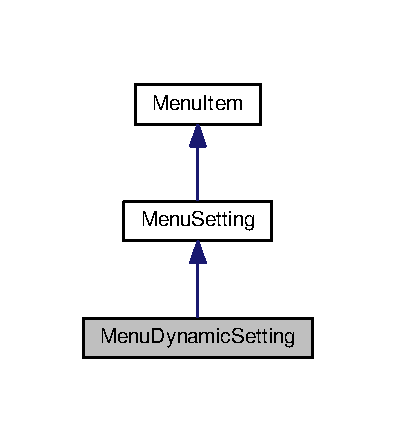
\includegraphics[width=190pt]{classMenuDynamicSetting__inherit__graph}
\end{center}
\end{figure}


Collaboration diagram for Menu\+Dynamic\+Setting\+:
\nopagebreak
\begin{figure}[H]
\begin{center}
\leavevmode
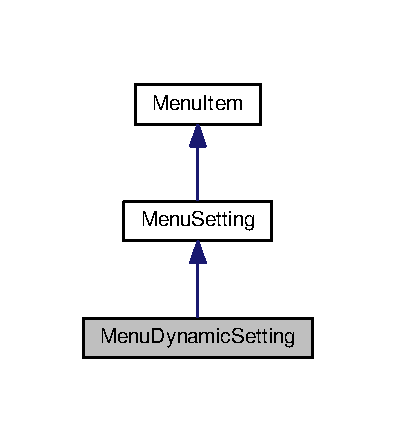
\includegraphics[width=190pt]{classMenuDynamicSetting__coll__graph}
\end{center}
\end{figure}
\subsection*{Additional Inherited Members}


\subsection{Detailed Description}
Dynamic Setting item, showing a list of values known only at runtime. 

This class holds a dynamic enum filled at runtime, for static values, use parent \hyperlink{classMenuSetting}{Menu\+Setting} 

The documentation for this class was generated from the following file\+:\begin{DoxyCompactItemize}
\item 
include/\hyperlink{MenuItem_8hh}{Menu\+Item.\+hh}\end{DoxyCompactItemize}

\hypertarget{classMenuEdit}{}\section{Menu\+Edit Class Reference}
\label{classMenuEdit}\index{Menu\+Edit@{Menu\+Edit}}


Input box, either used for key binding, or text input from user.  




{\ttfamily \#include $<$Menu\+Item.\+hh$>$}



Inheritance diagram for Menu\+Edit\+:\nopagebreak
\begin{figure}[H]
\begin{center}
\leavevmode
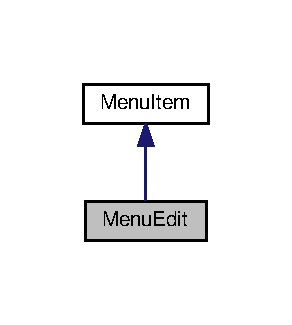
\includegraphics[width=140pt]{classMenuEdit__inherit__graph}
\end{center}
\end{figure}


Collaboration diagram for Menu\+Edit\+:\nopagebreak
\begin{figure}[H]
\begin{center}
\leavevmode
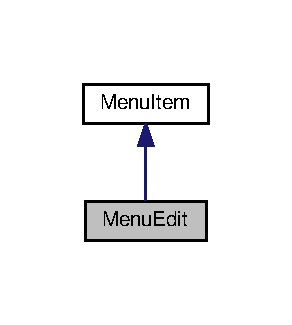
\includegraphics[width=140pt]{classMenuEdit__coll__graph}
\end{center}
\end{figure}
\subsection*{Additional Inherited Members}


\subsection{Detailed Description}
Input box, either used for key binding, or text input from user. 

This item is an input box to get a string from the user inside a \hyperlink{classMenu}{Menu}. 

The documentation for this class was generated from the following file\+:\begin{DoxyCompactItemize}
\item 
include/\hyperlink{MenuItem_8hh}{Menu\+Item.\+hh}\end{DoxyCompactItemize}

\hypertarget{classMenuItem}{}\section{Menu\+Item Class Reference}
\label{classMenuItem}\index{Menu\+Item@{Menu\+Item}}


Abstract \hyperlink{classMenu}{Menu} item.  




{\ttfamily \#include $<$Menu\+Item.\+hh$>$}



Inheritance diagram for Menu\+Item\+:
\nopagebreak
\begin{figure}[H]
\begin{center}
\leavevmode
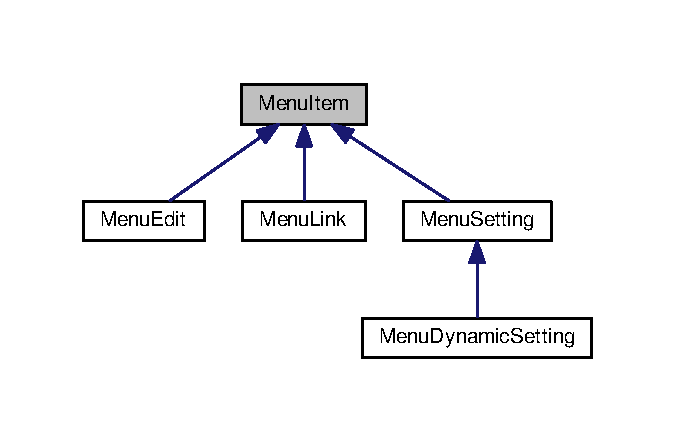
\includegraphics[width=324pt]{classMenuItem__inherit__graph}
\end{center}
\end{figure}
\subsection*{Public Member Functions}
\begin{DoxyCompactItemize}
\item 
{\bfseries Menu\+Item} (std\+::string \&)\hypertarget{classMenuItem_a07f74e3fc83f6a4aaef6675aef486e1d}{}\label{classMenuItem_a07f74e3fc83f6a4aaef6675aef486e1d}

\item 
void {\bfseries set\+Position} (sf\+::\+Vector2f \&pos)\hypertarget{classMenuItem_a58789909833868a64deb1b3a81f35ff4}{}\label{classMenuItem_a58789909833868a64deb1b3a81f35ff4}

\item 
virtual void {\bfseries on\+Click} (void $\ast$)=0\hypertarget{classMenuItem_a8be7ee76fe079bc6fee75d3d84a9db91}{}\label{classMenuItem_a8be7ee76fe079bc6fee75d3d84a9db91}

\end{DoxyCompactItemize}
\subsection*{Protected Attributes}
\begin{DoxyCompactItemize}
\item 
sf\+::\+Text {\bfseries \+\_\+label}\hypertarget{classMenuItem_ab0215e2c749d101cc1f3bda0801228c5}{}\label{classMenuItem_ab0215e2c749d101cc1f3bda0801228c5}

\end{DoxyCompactItemize}


\subsection{Detailed Description}
Abstract \hyperlink{classMenu}{Menu} item. 

This class is not instanciable. It is used as an abstract layer to store Items generically in \hyperlink{classMenu}{Menu} class. 

The documentation for this class was generated from the following file\+:\begin{DoxyCompactItemize}
\item 
include/\hyperlink{MenuItem_8hh}{Menu\+Item.\+hh}\end{DoxyCompactItemize}

\hypertarget{classMenuLink}{}\section{Menu\+Link Class Reference}
\label{classMenuLink}\index{Menu\+Link@{Menu\+Link}}


\hyperlink{classMenu}{Menu} link to another menu or action.  




{\ttfamily \#include $<$Menu\+Item.\+hh$>$}



Inheritance diagram for Menu\+Link\+:\nopagebreak
\begin{figure}[H]
\begin{center}
\leavevmode
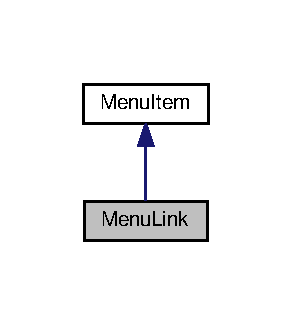
\includegraphics[width=140pt]{classMenuLink__inherit__graph}
\end{center}
\end{figure}


Collaboration diagram for Menu\+Link\+:\nopagebreak
\begin{figure}[H]
\begin{center}
\leavevmode
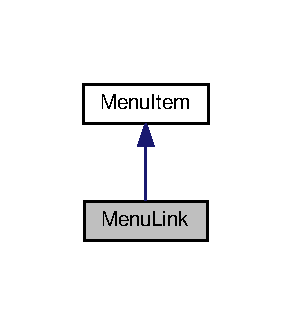
\includegraphics[width=140pt]{classMenuLink__coll__graph}
\end{center}
\end{figure}
\subsection*{Public Member Functions}
\begin{DoxyCompactItemize}
\item 
void {\bfseries on\+Click} ()\hypertarget{classMenuLink_a1242857c995165ecd13228f91662efc3}{}\label{classMenuLink_a1242857c995165ecd13228f91662efc3}

\end{DoxyCompactItemize}
\subsection*{Additional Inherited Members}


\subsection{Detailed Description}
\hyperlink{classMenu}{Menu} link to another menu or action. 

Link defines a \hyperlink{classMenuItem}{Menu\+Item} that is clickable and points towards another menu or do a specific action (quit, apply settings, ...) 

The documentation for this class was generated from the following file\+:\begin{DoxyCompactItemize}
\item 
include/\hyperlink{MenuItem_8hh}{Menu\+Item.\+hh}\end{DoxyCompactItemize}

\hypertarget{classMenuSetting}{}\section{Menu\+Setting Class Reference}
\label{classMenuSetting}\index{Menu\+Setting@{Menu\+Setting}}


Static Setting item, showing a list of values defined in X\+ML.  




{\ttfamily \#include $<$Menu\+Item.\+hh$>$}



Inheritance diagram for Menu\+Setting\+:
\nopagebreak
\begin{figure}[H]
\begin{center}
\leavevmode
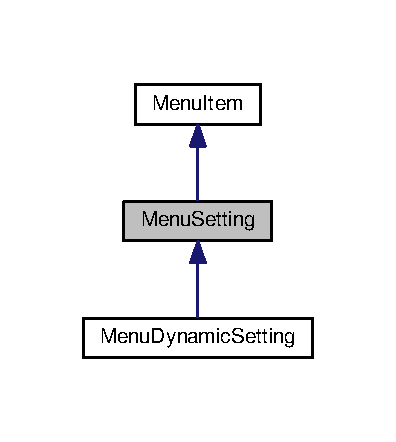
\includegraphics[width=190pt]{classMenuSetting__inherit__graph}
\end{center}
\end{figure}


Collaboration diagram for Menu\+Setting\+:\nopagebreak
\begin{figure}[H]
\begin{center}
\leavevmode
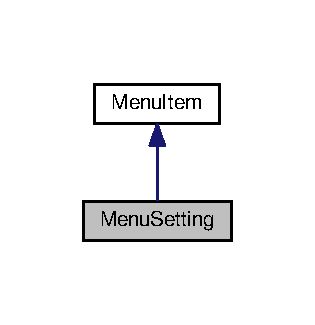
\includegraphics[width=151pt]{classMenuSetting__coll__graph}
\end{center}
\end{figure}
\subsection*{Additional Inherited Members}


\subsection{Detailed Description}
Static Setting item, showing a list of values defined in X\+ML. 

This class holds a static enum defined in X\+ML, for dynamic values, use child \hyperlink{classMenuDynamicSetting}{Menu\+Dynamic\+Setting} 

The documentation for this class was generated from the following file\+:\begin{DoxyCompactItemize}
\item 
include/\hyperlink{MenuItem_8hh}{Menu\+Item.\+hh}\end{DoxyCompactItemize}

\chapter{File Documentation}
\hypertarget{Commands_8hh}{}\section{include/\+Commands.hh File Reference}
\label{Commands_8hh}\index{include/\+Commands.\+hh@{include/\+Commands.\+hh}}


Contains definition of basic console commands.  


{\ttfamily \#include $<$map$>$}\\*
{\ttfamily \#include $<$vector$>$}\\*
Include dependency graph for Commands.\+hh\+:
\nopagebreak
\begin{figure}[H]
\begin{center}
\leavevmode
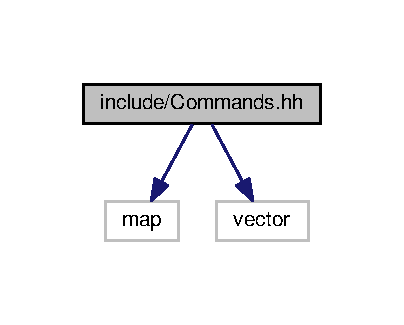
\includegraphics[width=194pt]{Commands_8hh__incl}
\end{center}
\end{figure}
This graph shows which files directly or indirectly include this file\+:
\nopagebreak
\begin{figure}[H]
\begin{center}
\leavevmode
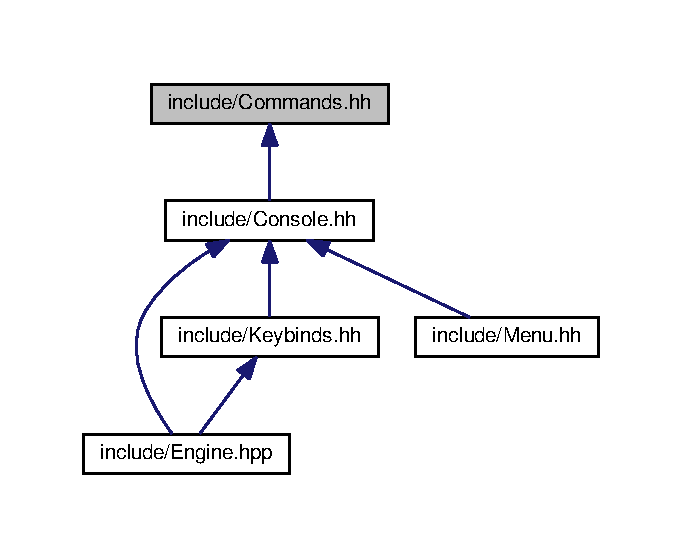
\includegraphics[width=194pt]{Commands_8hh__dep__incl}
\end{center}
\end{figure}
\subsection*{Typedefs}
\begin{DoxyCompactItemize}
\item 
typedef std\+::map$<$ std\+::string, void($\ast$)(\hyperlink{classEngine}{Engine} \&, std\+::vector$<$ std\+::string $>$ $\ast$)$>$ {\bfseries Commands\+::cmd\+Map}\hypertarget{Commands_8hh_a7d4b7cb98d97ada6d52d98d496d4645b}{}\label{Commands_8hh_a7d4b7cb98d97ada6d52d98d496d4645b}

\end{DoxyCompactItemize}
\subsection*{Functions}
\begin{DoxyCompactItemize}
\item 
bool {\bfseries Commands\+::convert\+Bool} (std\+::string \&arg)\hypertarget{Commands_8hh_abefc016d0d849fec28bcec9eb5c5b106}{}\label{Commands_8hh_abefc016d0d849fec28bcec9eb5c5b106}

\item 
std\+::vector$<$ std\+::string $>$ $\ast$ {\bfseries Commands\+::get\+Args} (std\+::string \&command)\hypertarget{Commands_8hh_aa0b47ec166c1143d0dd20c51b301e6af}{}\label{Commands_8hh_aa0b47ec166c1143d0dd20c51b301e6af}

\item 
bool {\bfseries Commands\+::parse\+Cmd} (\hyperlink{classEngine}{Engine} \&e, std\+::string)\hypertarget{Commands_8hh_a37f1ccb092695e87da41e0625b240bee}{}\label{Commands_8hh_a37f1ccb092695e87da41e0625b240bee}

\item 
void {\bfseries Commands\+::bind\+Command} (\hyperlink{classEngine}{Engine} \&e, std\+::vector$<$ std\+::string $>$ $\ast$)\hypertarget{Commands_8hh_ac98ddc07caa88b780eac831a7763db02}{}\label{Commands_8hh_ac98ddc07caa88b780eac831a7763db02}

\item 
void {\bfseries Commands\+::bind\+List} (\hyperlink{classEngine}{Engine} \&e, std\+::vector$<$ std\+::string $>$ $\ast$)\hypertarget{Commands_8hh_a6b9cff92e05b8ee3bbdf2183bcab0405}{}\label{Commands_8hh_a6b9cff92e05b8ee3bbdf2183bcab0405}

\item 
void {\bfseries Commands\+::console\+Clear} (\hyperlink{classEngine}{Engine} \&e, std\+::vector$<$ std\+::string $>$ $\ast$)\hypertarget{Commands_8hh_a1edaf40648864f95d6fabd821fa1ff69}{}\label{Commands_8hh_a1edaf40648864f95d6fabd821fa1ff69}

\item 
void {\bfseries Commands\+::console\+Toggle} (\hyperlink{classEngine}{Engine} \&e, std\+::vector$<$ std\+::string $>$ $\ast$)\hypertarget{Commands_8hh_a5ccaf75c545b581e6f56960a63789cc9}{}\label{Commands_8hh_a5ccaf75c545b581e6f56960a63789cc9}

\item 
void {\bfseries Commands\+::echo} (\hyperlink{classEngine}{Engine} \&e, std\+::vector$<$ std\+::string $>$ $\ast$)\hypertarget{Commands_8hh_acf0412f16ea578d5fa8a56804db65edf}{}\label{Commands_8hh_acf0412f16ea578d5fa8a56804db65edf}

\item 
void {\bfseries Commands\+::execute} (\hyperlink{classEngine}{Engine} \&e, std\+::vector$<$ std\+::string $>$ $\ast$)\hypertarget{Commands_8hh_a6cfb223a9b5b99372dd46ac74e45f05e}{}\label{Commands_8hh_a6cfb223a9b5b99372dd46ac74e45f05e}

\item 
void {\bfseries Commands\+::find\+Cmd} (\hyperlink{classEngine}{Engine} \&e, std\+::vector$<$ std\+::string $>$ $\ast$)\hypertarget{Commands_8hh_a5a9b5986047b6c3857a47309939338ea}{}\label{Commands_8hh_a5a9b5986047b6c3857a47309939338ea}

\item 
void {\bfseries Commands\+::toggle\+Con\+Log} (\hyperlink{classEngine}{Engine} \&, std\+::vector$<$ std\+::string $>$ $\ast$)\hypertarget{Commands_8hh_a29033c5de8eb9b3a459cce0af1b682e1}{}\label{Commands_8hh_a29033c5de8eb9b3a459cce0af1b682e1}

\item 
void {\bfseries Commands\+::write\+To\+Log} (\hyperlink{classEngine}{Engine} \&, std\+::vector$<$ std\+::string $>$ $\ast$argv)\hypertarget{Commands_8hh_abc6221d6db875de6393274c79050dc50}{}\label{Commands_8hh_abc6221d6db875de6393274c79050dc50}

\item 
void {\bfseries Commands\+::set\+Con\+Log} (\hyperlink{classEngine}{Engine} \&, std\+::vector$<$ std\+::string $>$ $\ast$argv)\hypertarget{Commands_8hh_a0b95e01fe5e51b1f1b7442169d22d016}{}\label{Commands_8hh_a0b95e01fe5e51b1f1b7442169d22d016}

\item 
void {\bfseries Commands\+::timestamp\+Log} (\hyperlink{classEngine}{Engine} \&, std\+::vector$<$ std\+::string $>$ $\ast$argv)\hypertarget{Commands_8hh_a02b2eb6659d7cf38798162dfae520105}{}\label{Commands_8hh_a02b2eb6659d7cf38798162dfae520105}

\item 
void {\bfseries Commands\+::print\+C\+WD} (\hyperlink{classEngine}{Engine} \&e, std\+::vector$<$ std\+::string $>$ $\ast$)\hypertarget{Commands_8hh_a78e83af80e189d307c49aa8db740b605}{}\label{Commands_8hh_a78e83af80e189d307c49aa8db740b605}

\item 
void {\bfseries Commands\+::quit} (\hyperlink{classEngine}{Engine} \&e, std\+::vector$<$ std\+::string $>$ $\ast$)\hypertarget{Commands_8hh_a25cfa3c76d0c7519d6fa7b3cee3bbd7d}{}\label{Commands_8hh_a25cfa3c76d0c7519d6fa7b3cee3bbd7d}

\item 
void {\bfseries Commands\+::screenshot} (\hyperlink{classEngine}{Engine} \&e, std\+::vector$<$ std\+::string $>$ $\ast$argv)\hypertarget{Commands_8hh_aa9cc2524a0648b744eedcb0714d89002}{}\label{Commands_8hh_aa9cc2524a0648b744eedcb0714d89002}

\item 
void {\bfseries Commands\+::set\+Line\+Count} (\hyperlink{classEngine}{Engine} \&e, std\+::vector$<$ std\+::string $>$ $\ast$)\hypertarget{Commands_8hh_a4bbf986e8df887b1eff58b289b1de43c}{}\label{Commands_8hh_a4bbf986e8df887b1eff58b289b1de43c}

\item 
void {\bfseries Commands\+::set\+Con\+Color} (\hyperlink{classEngine}{Engine} \&e, std\+::vector$<$ std\+::string $>$ $\ast$)\hypertarget{Commands_8hh_a555ae35c352b88fabdfc5626330ec99c}{}\label{Commands_8hh_a555ae35c352b88fabdfc5626330ec99c}

\item 
void {\bfseries Commands\+::set\+Con\+Cursor} (\hyperlink{classEngine}{Engine} \&e, std\+::vector$<$ std\+::string $>$ $\ast$)\hypertarget{Commands_8hh_a4794ec0d1c5f50648a2a402385d7a5f8}{}\label{Commands_8hh_a4794ec0d1c5f50648a2a402385d7a5f8}

\item 
void {\bfseries Commands\+::set\+Max\+F\+PS} (\hyperlink{classEngine}{Engine} \&e, std\+::vector$<$ std\+::string $>$ $\ast$)\hypertarget{Commands_8hh_a7255de2b4d70815909af4fe083683d25}{}\label{Commands_8hh_a7255de2b4d70815909af4fe083683d25}

\item 
void {\bfseries Commands\+::set\+Fullscreen} (\hyperlink{classEngine}{Engine} \&e, std\+::vector$<$ std\+::string $>$ $\ast$)\hypertarget{Commands_8hh_a95557710844e794e112337d7d6f7cdff}{}\label{Commands_8hh_a95557710844e794e112337d7d6f7cdff}

\item 
void {\bfseries Commands\+::help} (\hyperlink{classEngine}{Engine} \&e, std\+::vector$<$ std\+::string $>$ $\ast$)\hypertarget{Commands_8hh_ac172f253b5f32b4dddce8387fbc5c90f}{}\label{Commands_8hh_ac172f253b5f32b4dddce8387fbc5c90f}

\item 
void {\bfseries Commands\+::set\+V\+Sync} (\hyperlink{classEngine}{Engine} \&e, std\+::vector$<$ std\+::string $>$ $\ast$)\hypertarget{Commands_8hh_a403664e9d64fa9f76ae4e09d37dc86cd}{}\label{Commands_8hh_a403664e9d64fa9f76ae4e09d37dc86cd}

\item 
void {\bfseries Commands\+::unbind} (\hyperlink{classEngine}{Engine} \&e, std\+::vector$<$ std\+::string $>$ $\ast$)\hypertarget{Commands_8hh_aecb0f8c2aa97a861b3f7e096fa1c3753}{}\label{Commands_8hh_aecb0f8c2aa97a861b3f7e096fa1c3753}

\item 
void {\bfseries Commands\+::unbindall} (\hyperlink{classEngine}{Engine} \&e, std\+::vector$<$ std\+::string $>$ $\ast$)\hypertarget{Commands_8hh_aaf5fdc6ec45762f26fdd7c5edf9aeb55}{}\label{Commands_8hh_aaf5fdc6ec45762f26fdd7c5edf9aeb55}

\item 
void {\bfseries Commands\+::window\+Size} (\hyperlink{classEngine}{Engine} \&e, std\+::vector$<$ std\+::string $>$ $\ast$)\hypertarget{Commands_8hh_a1877584a3f78f6e917ad075f6f047c27}{}\label{Commands_8hh_a1877584a3f78f6e917ad075f6f047c27}

\end{DoxyCompactItemize}
\subsection*{Variables}
\begin{DoxyCompactItemize}
\item 
cmd\+Map {\bfseries Commands\+::cmdlist}\hypertarget{Commands_8hh_a858b3a3d3caa824a70c877892ff9e2a4}{}\label{Commands_8hh_a858b3a3d3caa824a70c877892ff9e2a4}

\end{DoxyCompactItemize}


\subsection{Detailed Description}
Contains definition of basic console commands. 

This file implements all the system console commands operations 
\hypertarget{Console_8hh}{}\section{include/\+Console.hh File Reference}
\label{Console_8hh}\index{include/\+Console.\+hh@{include/\+Console.\+hh}}
{\ttfamily \#include $<$list$>$}\\*
{\ttfamily \#include $<$deque$>$}\\*
{\ttfamily \#include $<$fstream$>$}\\*
{\ttfamily \#include $<$S\+F\+M\+L/\+Graphics.\+hpp$>$}\\*
{\ttfamily \#include \char`\"{}Commands.\+hh\char`\"{}}\\*
Include dependency graph for Console.\+hh\+:
\nopagebreak
\begin{figure}[H]
\begin{center}
\leavevmode
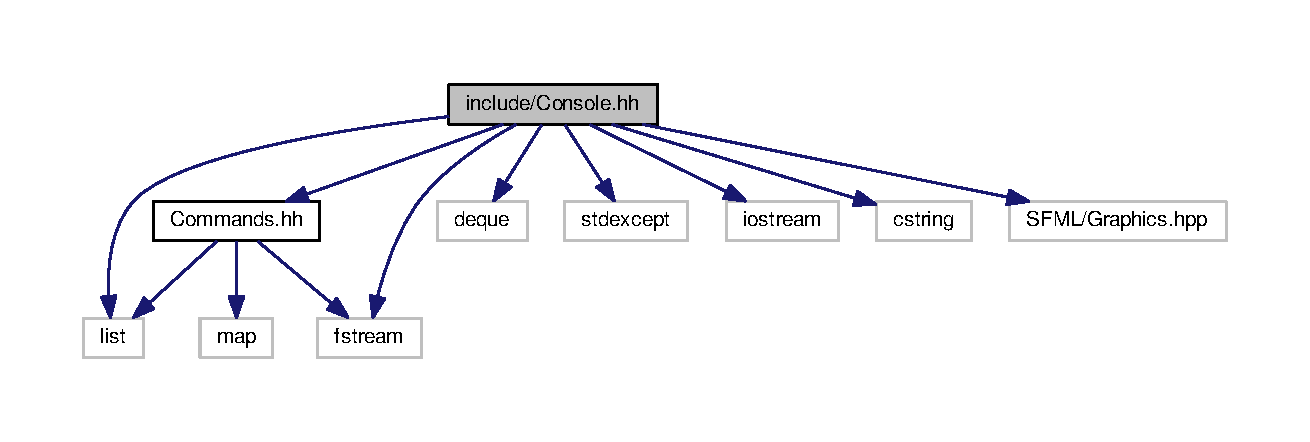
\includegraphics[width=350pt]{Console_8hh__incl}
\end{center}
\end{figure}
This graph shows which files directly or indirectly include this file\+:
\nopagebreak
\begin{figure}[H]
\begin{center}
\leavevmode
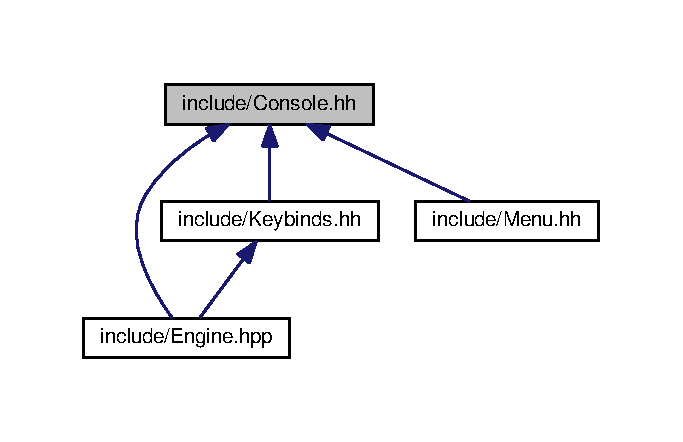
\includegraphics[width=180pt]{Console_8hh__dep__incl}
\end{center}
\end{figure}
\subsection*{Classes}
\begin{DoxyCompactItemize}
\item 
class \hyperlink{classConsole}{Console}
\begin{DoxyCompactList}\small\item\em Integrated toggleable developer console. \end{DoxyCompactList}\end{DoxyCompactItemize}
\subsection*{Macros}
\begin{DoxyCompactItemize}
\item 
\#define {\bfseries P\+R\+O\+M\+PT}~(\char`\"{}$>$\char`\"{})\hypertarget{Console_8hh_accdbea14ea06c15e271784368bd993e8}{}\label{Console_8hh_accdbea14ea06c15e271784368bd993e8}

\item 
\#define {\bfseries C\+U\+R\+S\+OR}~(\char`\"{}\+\_\+\char`\"{})\hypertarget{Console_8hh_ae67dffdc8e496c16aff7e8903a3f2117}{}\label{Console_8hh_ae67dffdc8e496c16aff7e8903a3f2117}

\item 
\#define {\bfseries C\+O\+L\+O\+R\+\_\+\+E\+SC}~(\char`\"{}\textbackslash{}\textbackslash{}\textbackslash{}\textbackslash{}\#\char`\"{})\hypertarget{Console_8hh_ad35272f2bff654b0397a96776e9fc8b4}{}\label{Console_8hh_ad35272f2bff654b0397a96776e9fc8b4}

\item 
\#define {\bfseries C\+O\+L\+O\+R\+\_\+\+E\+R\+R\+OR}~(\char`\"{}\textbackslash{}\textbackslash{}\textbackslash{}\textbackslash{}\#240077077\char`\"{})\hypertarget{Console_8hh_ac7bab6591a09366d23b86d710ecc54af}{}\label{Console_8hh_ac7bab6591a09366d23b86d710ecc54af}

\item 
\#define {\bfseries C\+O\+L\+O\+R\+\_\+\+S\+U\+C\+C\+E\+SS}~(\char`\"{}\textbackslash{}\textbackslash{}\textbackslash{}\textbackslash{}\#154205050\char`\"{})\hypertarget{Console_8hh_a49ad0d2196700c1fa0a3a2a60dad41d3}{}\label{Console_8hh_a49ad0d2196700c1fa0a3a2a60dad41d3}

\item 
\#define {\bfseries C\+O\+L\+O\+R\+\_\+\+I\+N\+FO}~(\char`\"{}\textbackslash{}\textbackslash{}\textbackslash{}\textbackslash{}\#000191255\char`\"{})\hypertarget{Console_8hh_a0d4d3a685f9501631d1feed1f4ba7577}{}\label{Console_8hh_a0d4d3a685f9501631d1feed1f4ba7577}

\item 
\#define {\bfseries C\+U\+R\+S\+O\+R\+\_\+\+D\+E\+L\+AY}~(500)\hypertarget{Console_8hh_a59178e92910e3e77a4714bb1ced95909}{}\label{Console_8hh_a59178e92910e3e77a4714bb1ced95909}

\end{DoxyCompactItemize}

\hypertarget{Control_8hh}{}\section{include/\+Control.hh File Reference}
\label{Control_8hh}\index{include/\+Control.\+hh@{include/\+Control.\+hh}}
{\ttfamily \#include $<$S\+F\+M\+L/\+Graphics.\+hpp$>$}\\*
Include dependency graph for Control.\+hh\+:\nopagebreak
\begin{figure}[H]
\begin{center}
\leavevmode
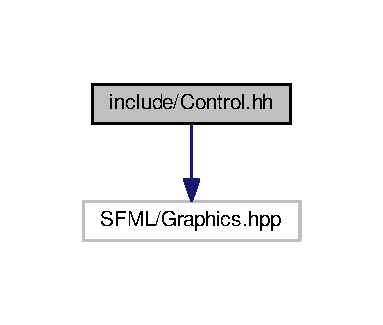
\includegraphics[width=184pt]{Control_8hh__incl}
\end{center}
\end{figure}
This graph shows which files directly or indirectly include this file\+:\nopagebreak
\begin{figure}[H]
\begin{center}
\leavevmode
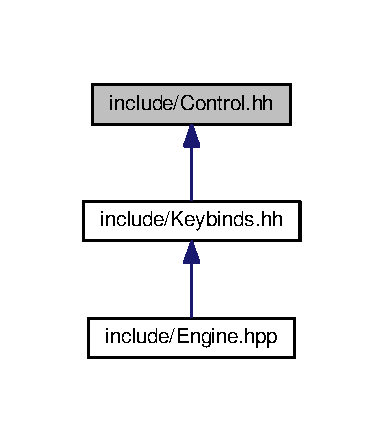
\includegraphics[width=184pt]{Control_8hh__dep__incl}
\end{center}
\end{figure}
\subsection*{Classes}
\begin{DoxyCompactItemize}
\item 
class \hyperlink{classControl}{Control}
\begin{DoxyCompactList}\small\item\em Key, or Mouse event. \end{DoxyCompactList}\end{DoxyCompactItemize}
\subsection*{Enumerations}
\begin{DoxyCompactItemize}
\item 
enum {\bfseries Control\+Type} \{ {\bfseries Null}, 
{\bfseries Key}, 
{\bfseries M\+Button}, 
{\bfseries M\+Wheel}
 \}\hypertarget{Control_8hh_a8005f1f182fd0248a710ca64f72508d4}{}\label{Control_8hh_a8005f1f182fd0248a710ca64f72508d4}

\item 
enum {\bfseries Wheel\+Move} \{ {\bfseries Up} = -\/1, 
{\bfseries Down} = 1
 \}\hypertarget{Control_8hh_ad869e3b0cbdf01650550be2582e42c1e}{}\label{Control_8hh_ad869e3b0cbdf01650550be2582e42c1e}

\end{DoxyCompactItemize}

\hypertarget{Engine_8hpp}{}\section{include/\+Engine.hpp File Reference}
\label{Engine_8hpp}\index{include/\+Engine.\+hpp@{include/\+Engine.\+hpp}}
{\ttfamily \#include $<$S\+F\+M\+L/\+Graphics.\+hpp$>$}\\*
{\ttfamily \#include \char`\"{}Console.\+hh\char`\"{}}\\*
{\ttfamily \#include \char`\"{}Keybinds.\+hh\char`\"{}}\\*
Include dependency graph for Engine.\+hpp\+:
\nopagebreak
\begin{figure}[H]
\begin{center}
\leavevmode
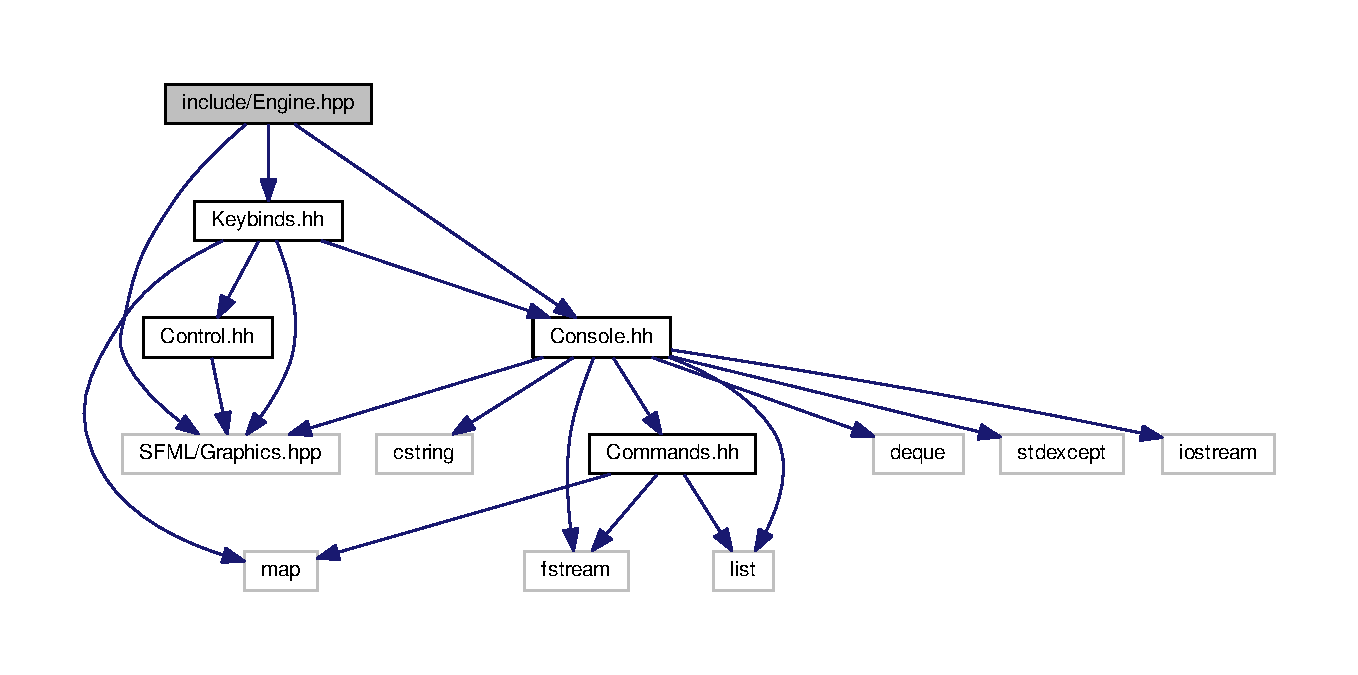
\includegraphics[width=350pt]{Engine_8hpp__incl}
\end{center}
\end{figure}
\subsection*{Classes}
\begin{DoxyCompactItemize}
\item 
class \hyperlink{classEngine}{Engine}
\begin{DoxyCompactList}\small\item\em Main class for graphic conception. \end{DoxyCompactList}\end{DoxyCompactItemize}
\subsection*{Enumerations}
\begin{DoxyCompactItemize}
\item 
enum {\bfseries Char\+Type} \{ {\bfseries alphanumeric}, 
{\bfseries alphabetic}, 
{\bfseries numeric}
 \}\hypertarget{Engine_8hpp_a29966b9994a4b4e8c250133a79f4a2e0}{}\label{Engine_8hpp_a29966b9994a4b4e8c250133a79f4a2e0}

\end{DoxyCompactItemize}

\hypertarget{Keybinds_8hh}{}\section{include/\+Keybinds.hh File Reference}
\label{Keybinds_8hh}\index{include/\+Keybinds.\+hh@{include/\+Keybinds.\+hh}}
{\ttfamily \#include $<$S\+F\+M\+L/\+Graphics.\+hpp$>$}\\*
{\ttfamily \#include $<$map$>$}\\*
{\ttfamily \#include \char`\"{}Console.\+hh\char`\"{}}\\*
{\ttfamily \#include \char`\"{}Control.\+hh\char`\"{}}\\*
Include dependency graph for Keybinds.\+hh\+:\nopagebreak
\begin{figure}[H]
\begin{center}
\leavevmode
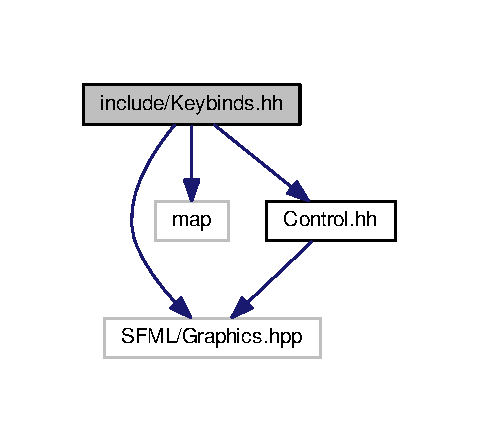
\includegraphics[width=350pt]{Keybinds_8hh__incl}
\end{center}
\end{figure}
This graph shows which files directly or indirectly include this file\+:\nopagebreak
\begin{figure}[H]
\begin{center}
\leavevmode
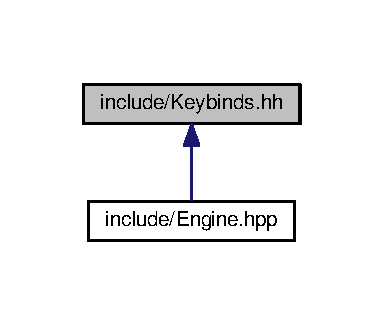
\includegraphics[width=184pt]{Keybinds_8hh__dep__incl}
\end{center}
\end{figure}
\subsection*{Classes}
\begin{DoxyCompactItemize}
\item 
class \hyperlink{classKeybinds}{Keybinds}
\begin{DoxyCompactList}\small\item\em Dictionnary of current bound keys at runtime. \end{DoxyCompactList}\end{DoxyCompactItemize}
\subsection*{Macros}
\begin{DoxyCompactItemize}
\item 
\#define {\bfseries B\+I\+N\+D\+R\+EF}(x)~(Engine\+::keybinds-\/$>$get\+Key(x))\hypertarget{Keybinds_8hh_aa97e65a268c7b74ecb84e324ee948be2}{}\label{Keybinds_8hh_aa97e65a268c7b74ecb84e324ee948be2}

\item 
\#define {\bfseries B\+I\+N\+D\+T\+R\+I\+G\+G\+E\+R\+ED}(x,  evn)~(Engine\+::keybinds-\/$>$get\+Key(x)-\/$>$is\+Triggered(evn))\hypertarget{Keybinds_8hh_a20735dc5e19dc878fa8b684e85042adb}{}\label{Keybinds_8hh_a20735dc5e19dc878fa8b684e85042adb}

\end{DoxyCompactItemize}

\hypertarget{Menu_8hh}{}\section{include/\+Menu.hh File Reference}
\label{Menu_8hh}\index{include/\+Menu.\+hh@{include/\+Menu.\+hh}}
{\ttfamily \#include $<$S\+F\+M\+L/\+Graphics.\+hpp$>$}\\*
{\ttfamily \#include \char`\"{}Menu\+Item.\+hh\char`\"{}}\\*
Include dependency graph for Menu.\+hh\+:
\nopagebreak
\begin{figure}[H]
\begin{center}
\leavevmode
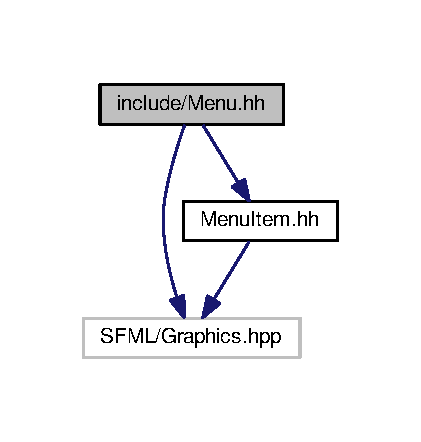
\includegraphics[width=202pt]{Menu_8hh__incl}
\end{center}
\end{figure}
\subsection*{Classes}
\begin{DoxyCompactItemize}
\item 
class \hyperlink{classMenu}{Menu}
\begin{DoxyCompactList}\small\item\em Simple class for generating menus. \end{DoxyCompactList}\end{DoxyCompactItemize}
\subsection*{Typedefs}
\begin{DoxyCompactItemize}
\item 
typedef std\+::vector$<$ \hyperlink{classMenuItem}{Menu\+Item} $\ast$ $>$ {\bfseries item\+Tab}\hypertarget{Menu_8hh_a9ad12c681980730aa31035398264e44b}{}\label{Menu_8hh_a9ad12c681980730aa31035398264e44b}

\end{DoxyCompactItemize}

\hypertarget{MenuItem_8hh}{}\section{include/\+Menu\+Item.hh File Reference}
\label{MenuItem_8hh}\index{include/\+Menu\+Item.\+hh@{include/\+Menu\+Item.\+hh}}


\hyperlink{classMenu}{Menu} items (links, settings, sliders, text inputs, ...)  


{\ttfamily \#include $<$S\+F\+M\+L/\+Graphics.\+hpp$>$}\\*
Include dependency graph for Menu\+Item.\+hh\+:\nopagebreak
\begin{figure}[H]
\begin{center}
\leavevmode
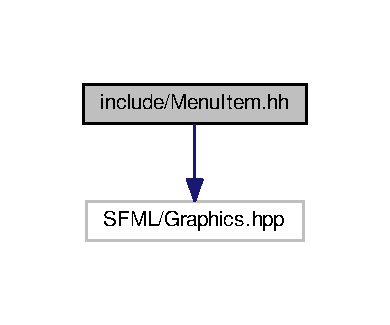
\includegraphics[width=187pt]{MenuItem_8hh__incl}
\end{center}
\end{figure}
\subsection*{Classes}
\begin{DoxyCompactItemize}
\item 
class \hyperlink{classMenuItem}{Menu\+Item}
\begin{DoxyCompactList}\small\item\em Abstract \hyperlink{classMenu}{Menu} item. \end{DoxyCompactList}\item 
class \hyperlink{classMenuLink}{Menu\+Link}
\begin{DoxyCompactList}\small\item\em \hyperlink{classMenu}{Menu} link to another menu or action. \end{DoxyCompactList}\item 
class \hyperlink{classMenuSetting}{Menu\+Setting}
\begin{DoxyCompactList}\small\item\em Static Setting item, showing a list of values defined in X\+ML. \end{DoxyCompactList}\item 
class \hyperlink{classMenuDynamicSetting}{Menu\+Dynamic\+Setting}
\begin{DoxyCompactList}\small\item\em Dynamic Setting item, showing a list of values known only at runtime. \end{DoxyCompactList}\item 
class \hyperlink{classMenuEdit}{Menu\+Edit}
\begin{DoxyCompactList}\small\item\em Input box, either used for key binding, or text input from user. \end{DoxyCompactList}\end{DoxyCompactItemize}


\subsection{Detailed Description}
\hyperlink{classMenu}{Menu} items (links, settings, sliders, text inputs, ...) 

This classes set provide usables objects for all kinds of items in a menu. It defines Links, Settings, and Edit types,which are specialized in child objects like Sliders, Static and Dynamic enums for Settings, and Key or String for Edit. 
%--- End generated contents ---

% Index
\backmatter
\newpage
\phantomsection
\clearemptydoublepage
\addcontentsline{toc}{chapter}{Index}
\printindex

\end{document}
